\chapter{Riemann Pump Circuit design}
\label{ch:design}
\textit{Description of the approach you have taken to solve the scientific or technical problem which you were posed. Outline the design, the methodology and overall structure of your experimental approach}\\ 
After a literature survey on the topic of the Riemann Pump and the corresponding high speed \gls{ab:dac} an approach is chosen to implement which seems to fulfill the most of the characteristic parameters \ref{ch:characteristics}.
This concept of push-pull stage seems to fit the best in a simple way with elements already used... -> verified, validated, tested, measured,...
In addition to this parameters the realised approach is a first, easy to implement way to design such a complex system.
Since the scope of the thesis is limited to time issues and there was no time for a stand alone design and redesign an already known concept of D. Maksimovic \cite{MaksimovicPaper} is used.

The concept of the Riemann Pump as seen in Fig. \ref{fig:RiemannPumpConcept} is realised with the design tool \gls{ab:ads}.
The first step was to design a 
A digitally controlled charge pump with eight different slopes is created, called Riemann Pump. To show that this pump is able to convert a digital signal into an analog one an example code is generated. As a MATLAB algorithm do not exists, which computes the Riemann Code, it is done by hand.
In fact of the high energy consumption, the realized DAC is designed for the integration in a base station. Because it converts a digital bit sequence into an analog rf signal it is implemented in the transmitting path. Based on the idea of a push-pull stage the load impedance of the charge pump is designed first.
\section{Approach and implementation of the Riemann Pump}
One possible approach to design a charge pump as shown in Fig. \ref{fig:RiemannPumpConcept} was with concept of a Push-Pull stage.
The concept of the chosen push-pull stage had the advantage of an integrated driver circuit which allows to switch the high side transistor efficient.
This concept is usually used for power electronics [-> which power electronic, refer to].
The first approach of designing a Riemann Pump was with a concept of a Push-Pull stage. This push-pull stage should charge a capacitive load at the output, which is the same as a normal charge pump. Push-pull stages complementary switch a high- and lowside transistor as in a charge pump. This was one possible approach. Concept of Maksimovic.

%\begin{figure}[ht]
%	\centering
%  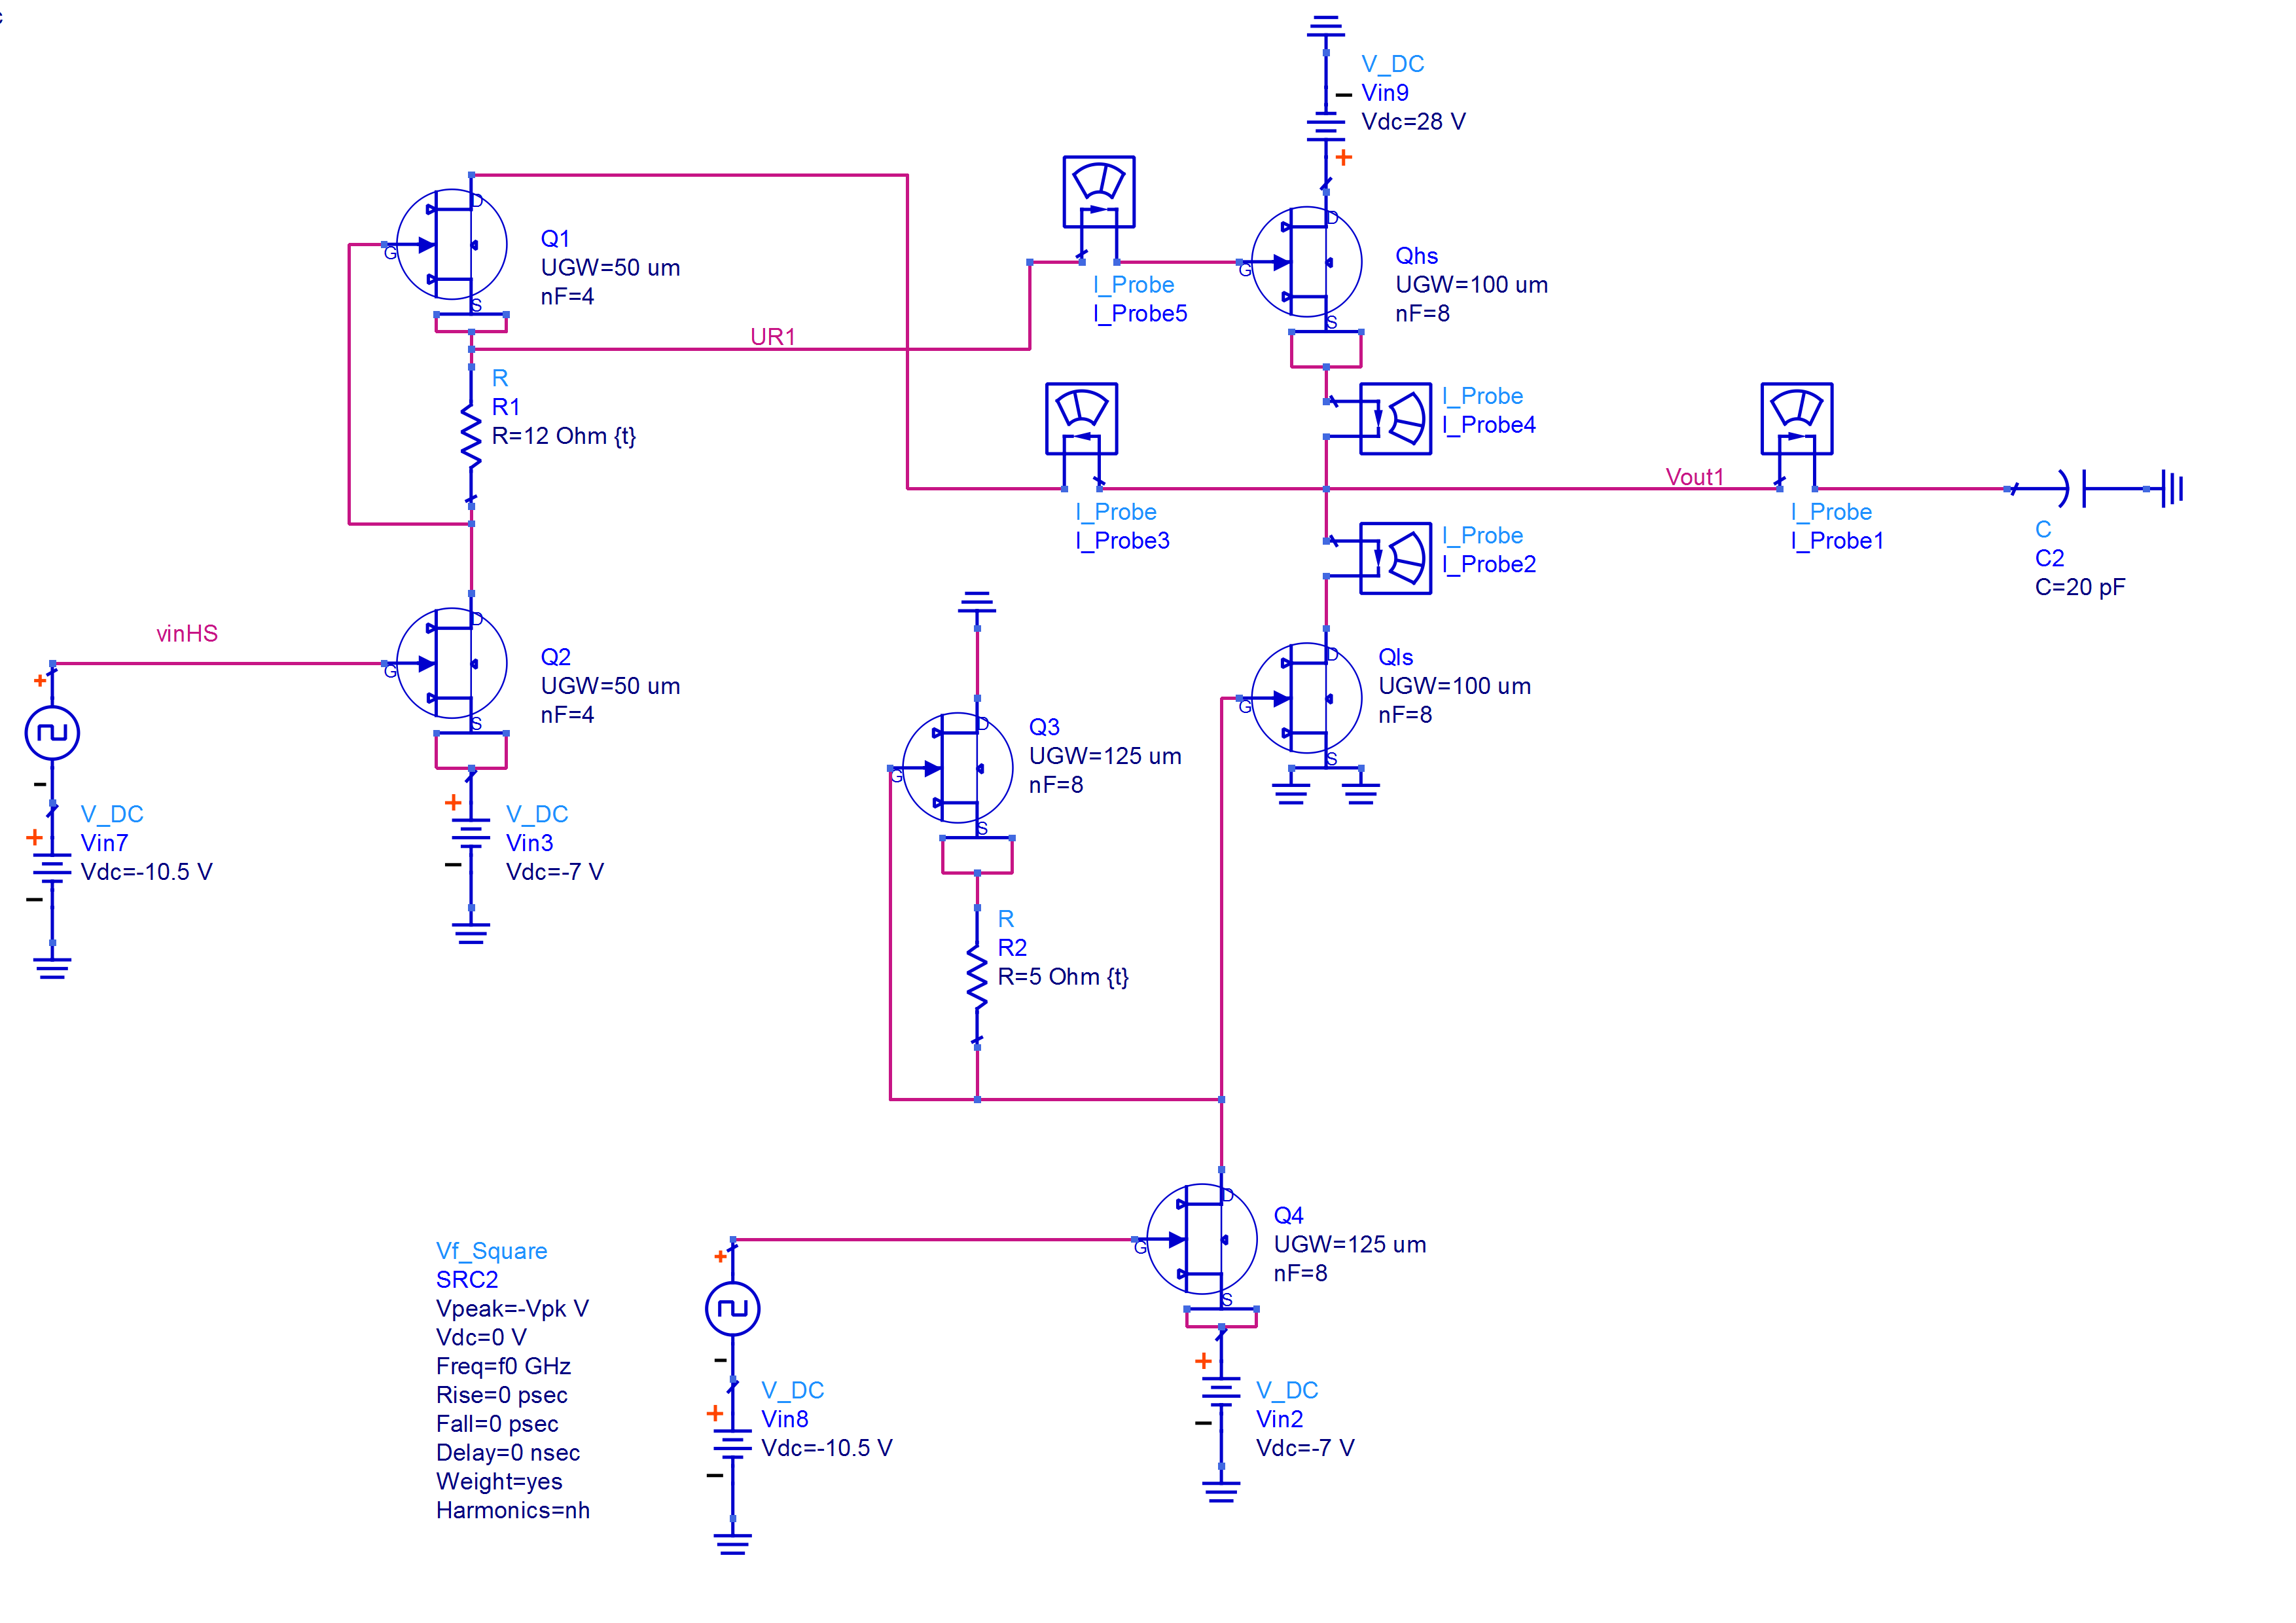
\includegraphics[width=1\textwidth]{Active_PullUp3.png}
%	\caption{Schematic of a driver circuit with push-pull stage representing one bit of the DAC called Riemann Pump}
%	\label{RiemannPump}
%\end{figure}



\begin{figure}[ht]
	\centering
  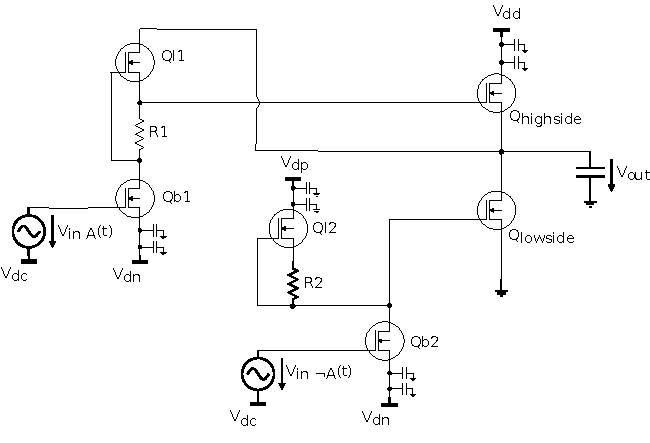
\includegraphics[width=1\textwidth]{Schematic_RP_concept.pdf}
	\caption{Schematic of a push-pull stage with corresponding driver representing one bit of the Riemann Pump}
	\label{RiemannPump}
\end{figure}

%
%\begin{figure}[htb!]
%   \centering 
%   \input{graphics/concept/Schematic_RP_concept.pdf_tex}
%   \caption{Schematic of the Riemann Pump circuit}
%   \label{fig:RiemannCodeGenerationSineWave}
%\end{figure} 
 
 
 
 


\section{Identification of the load impedance}
To proof the concept of the chosen approach an appropriate output impedance was needed to synthesize the desired signal.
The suitable output impedance was identified using the assumption to drive a power amplifier with the synthesized signal.

\textbf{The advantage to drive a power amplifier with the synthesized signal would be... to synthesize a signal near to the RF- front end e.g. in a base station for mobile communication. - paper why this is needed}
As a \SI{20}{\watt} power amplifier would be taken for the transmitting path of a base station the corresponding gate periphery of a \gls{ab:gan}25 transistor would be \SI{4}{\milli \metre}.
This is a keep it small and simple approach to get a first idea of the concept. Otherwise a more accurate way would be to take a broadband power amplifier as load.
The transistor model with this gate periphery was tuned due to the \gls{ab:mag} to get the complex impedance of the power amplifier.
After the tuning process a S-parameter simulation determined the input impedance of the power amplifier which corresponds to the load impedance of the designed Riemann pump circuit.
This transistor model \gls{ab:hemt} (IAF\_GE\_MSL\_ A204/IAF\_GaN25\_HEMT\_CS\_LS\_SHfull) used in \gls{ab:ads} were modelled at the \gls{ab:iaf}.\\

 The first assumption is that the load is a pre-power amplifier which generate a power of \SI{20}{\watt}. To generate this power, the gate periphery of a GaN25 HEMT has to be \SI{4}{\milli \metre} based on the approximation(- official reference???) \SI[per-mode=fraction]{5}{\watt\per\milli\metre}. To get this gate periphery four transistor in parallel each with 8 finger and \SI{125}{\micro \metre} are designed for the power amplifier. The bias point is determined with the \gls{ab:mag}. Therefore the following load impedance could be determined.
\begin{equation}
Z = R - jX_c
\end{equation}

With the help of the $S_{11}$ parameter plotted in the smith chart Fig. \ref{fig:smith_load_impedance} the load impedance can be determined.
The load impedance got a capacitive reactance.
 The real part of the impedance is roughly $R = \SI{1.89}{\ohm}$, while the imaginary part is capacitive. An important point is the input capacitance is increasing with frequency. While it is normal that the imaginary part of the impedance is increasing with frequency, the input capacitance is not.

 \begin{figure}[ht]
	\centering
  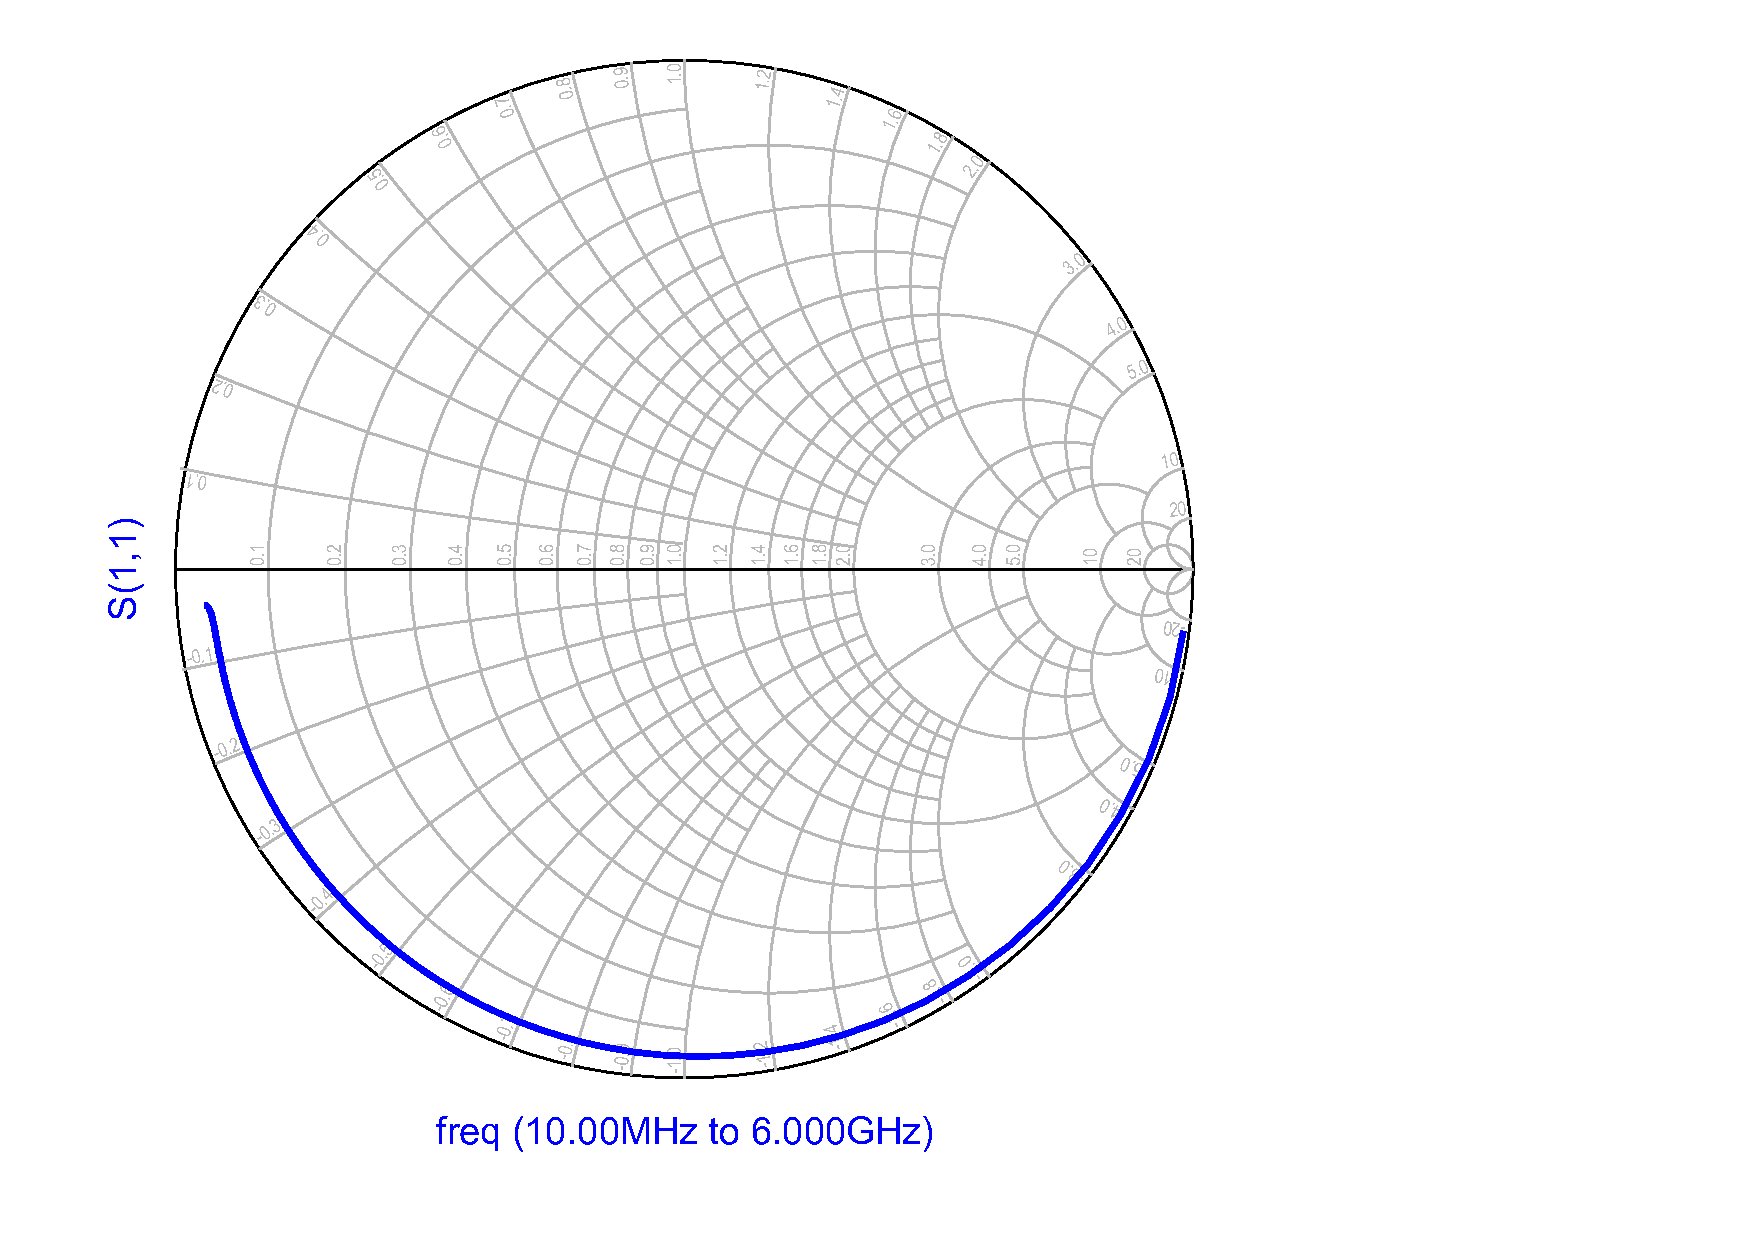
\includegraphics[width=1\textwidth]{S_param_LoadImpedance.pdf}
	\caption{smith chart representing the load impedance}
	\label{fig:smith_load_impedance}
\end{figure}

The load capacitance is calculated through the complex impedance:
\begin{equation}
C = \frac{1}{2 \pi f X_c}
\end{equation}

 \begin{figure}[ht]
	\centering
  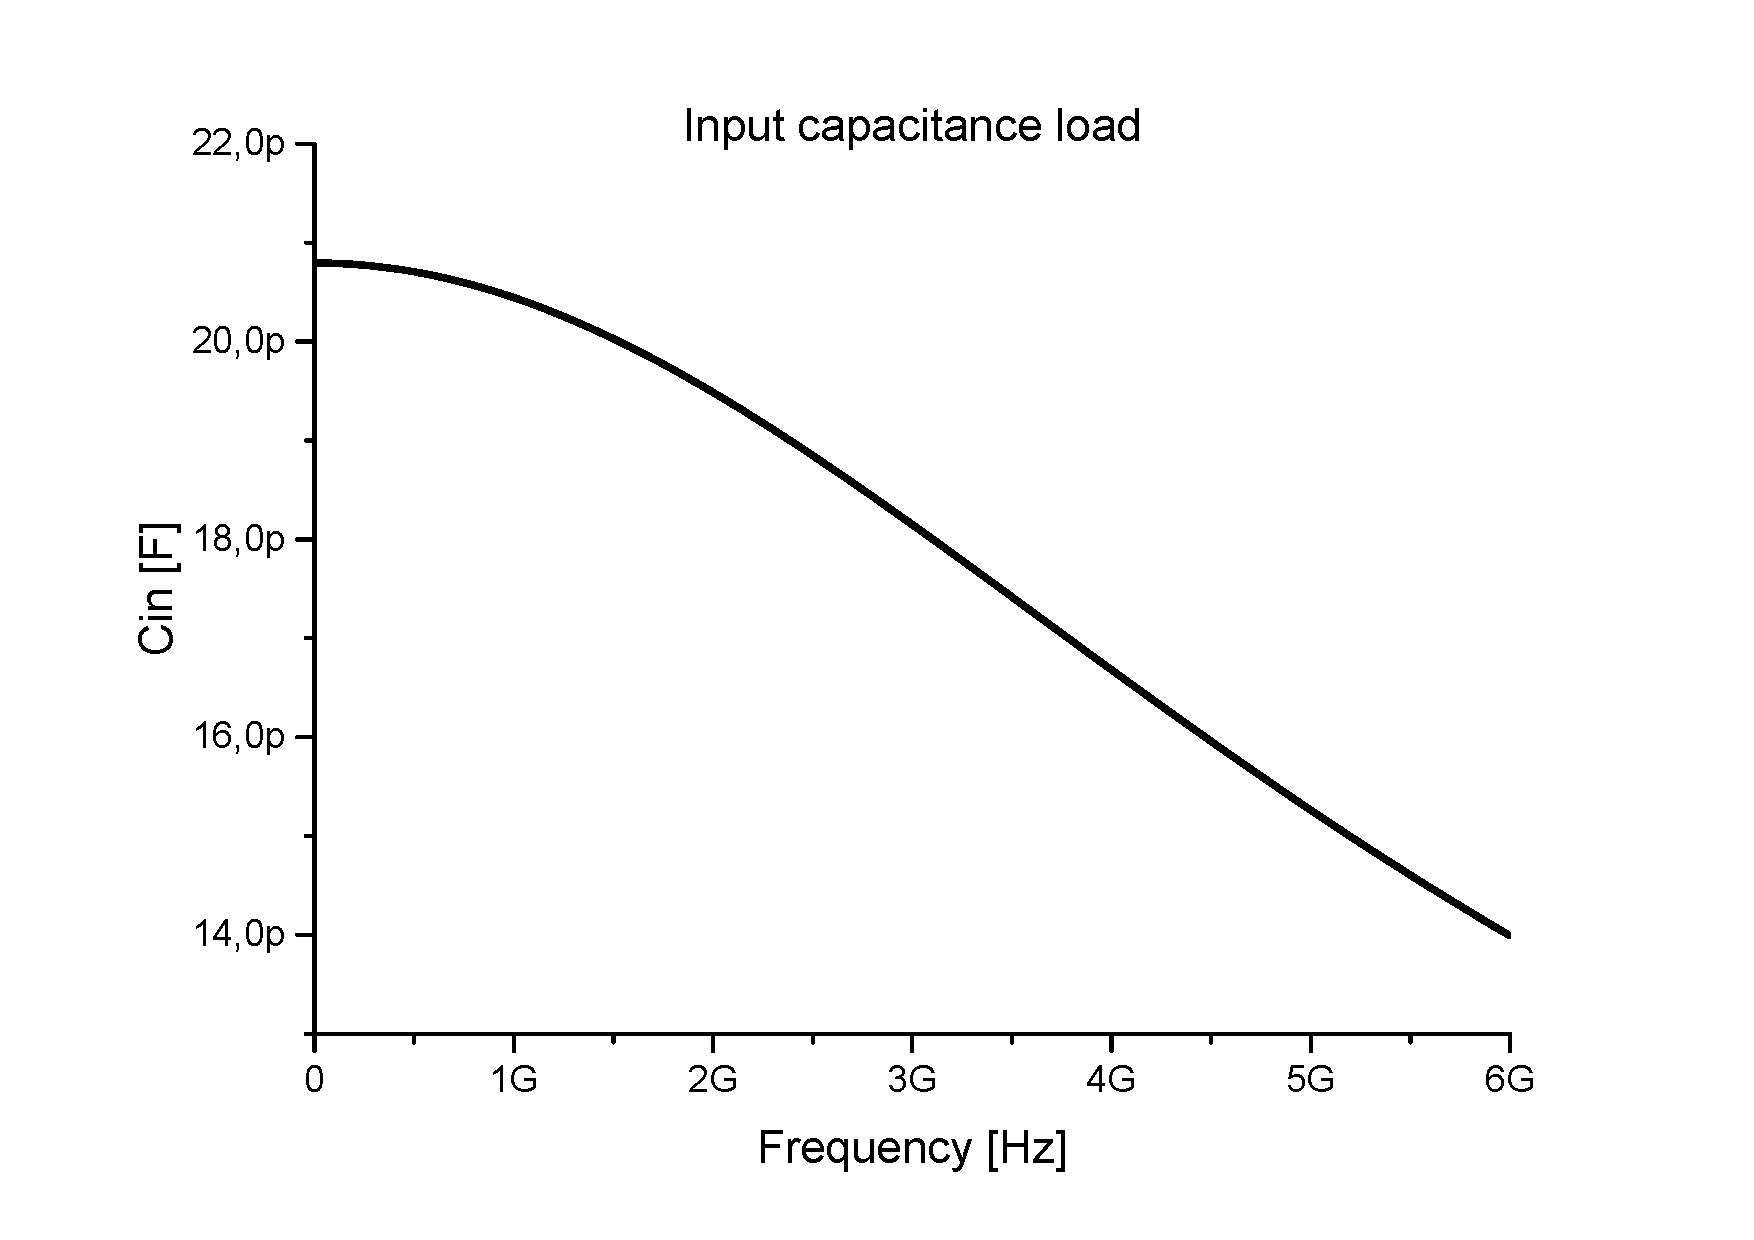
\includegraphics[width=0.5\textwidth]{InputCap_LoadImpedance_6GHz.pdf}
	\caption{frequency dependent input capacitance of the load}
	\label{fig:smith_load_impedance_inC}
\end{figure}

\section{Dimension of the used components}
The transistor dimension were... Different for driver circuit and power circuit... resistor to reduce the energy  consumption, for higher efficiency. \\ The
approach of the push-pull stage Maksimovic, Maroldt.\\
Approach of theoretical and synthesized signal -> MatLab generation of Riemanncode, SNR.\\ Stability, driver concept, energy consumption, frequency bandwidth, gain
Schematic design in Advanced Design System 2014. concept, ideas... 
\textbf{length of the bonds, number of bonds, thickness of bonds ask Dirk Meder. A lot of vias - more inductance - voltage drop between layers. short as possible lines, no rechtecke - para caps in the edge. first filter cap to supply pin near the chip. number and cap size determined on experience. }\\
Control voltage of 5 V realization with OPAMPS? Possible to overdrive opamps instead of using broadband ppa. 


\section{Circuit design summary and discussion}
\textit{Drawbacks, problems, challenges.}
Same realisation problems and difficulties: Problem of BANDWIDTH, Vpp of control signal (5V pp for GaN transistors), high side driver, no complementary transistors available in III-V technology, low loss driver, high speed driver, digital control driver, too high energy consumption (stability???)
\textbf{bandwidth limitation}
\textit{The lower bound is determined by the sampling time (inverse of the sampling frequency) and the smallest current achieved with the dimensioned transistors.
 The smallest achievable current times the smallest sampling time (highest sampling frequency) determine the smallest absolute slope achievable. \\
 \textbf{Is every signal possible to create?$\rightarrow$ a rect signal has too steep flanks to create. The signal bandwidth ranges from DC to 6 GHz but what is the amplitude range? Is there a limitation regarding the amplitude?}
\\
The smallest current is determined by the dimension of the transistor, which drives into saturation. 
The smallest saturated current is determined by the push-pull transistor geometry, here: 532 mA.}